\section{Webapplikation}
Applikationen er integrationstestet med test frameworket Jasmine og Protractor\footnote{http://angular.github.io/protractor/}. Protractor er et node.js test framework som google har udviklet specielt til test af AngularJS applikationer. Testene bliver afviklet på en test server som går ind på webapplikationen og simulere brugen af applikationen. Protractor skal bruge to filer for at kunne udføre tests på applikationen.\linebreak

\textbf{protractor.conf.js}\\
Config filen skal bruges til at køre testene. Her bestemmes hvilke test server der skal benyttes til at udføre testene på, hvor test filerne ligger, browser type osv. Som standart bruger Protractor chrome som test browser. I config filen er rootElement også sat, hvilket bruges til at fortælle Protractor at testene ikke skal begynde for projektets rootElement er loaded. 

\textbf{test fil}\\
Det sidste protractor skal bruge for at kunne køre her en test fil eller flere test filer som skal afvikles. 

\subsection{Kør tests}
For at testene kan afvikles skal først test serveren startes. Dette gøres via commandoen:

\begin{lstlisting}[language=bash]
	$ webdriver-manager start
\end{lstlisting}

Efter denne kommando starter test serveren op. Og nu kan testene afvikles ved kommandoen:

\begin{lstlisting}[language=bash]
	$ protractor protractor.conf.js
\end{lstlisting}

På figur \ref{fig:integration_exampel} ses et udsnit af integrations test outputtet.

\vspace{-5pt}
%kommentar
\begin{figure}[H]
	\centering
	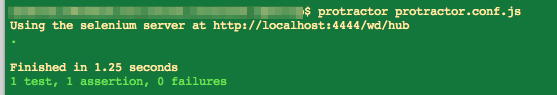
\includegraphics[width=0.7\textwidth]{Billeder/Test/integration_web.png}
	\vspace{-5pt}
	\caption{Test eksempel}
	\label{fig:integration_exampel}
\end{figure}

Yderligere information omkring test kan findes i test filerne i mappen test under integrations test som ligger i roden af projektet.